Mecanum wheels, a distinctive omnidirectional wheel design, enable vehicles to maneuver freely in any direction, including forward, backward, laterally, and rotationally. This unique capability is achieved through the arrangement of rollers on the wheel, which are mounted at an angle to the wheel's axis. The side view of such an wheel can be seen in fig.~\ref{fig:mecanumwheel}. Unlike conventional wheeled systems, which are limited to two degrees of freedom (longitudinal and steering), Mecanum wheels provide full omnidirectional movement with three \ac{dof}: longitudinal, lateral, and rotational (yaw)~\cite{Dickerson.1991}.\\
\begin{figure}[h]
	\centering
	\captionsetup{justification=centering}
	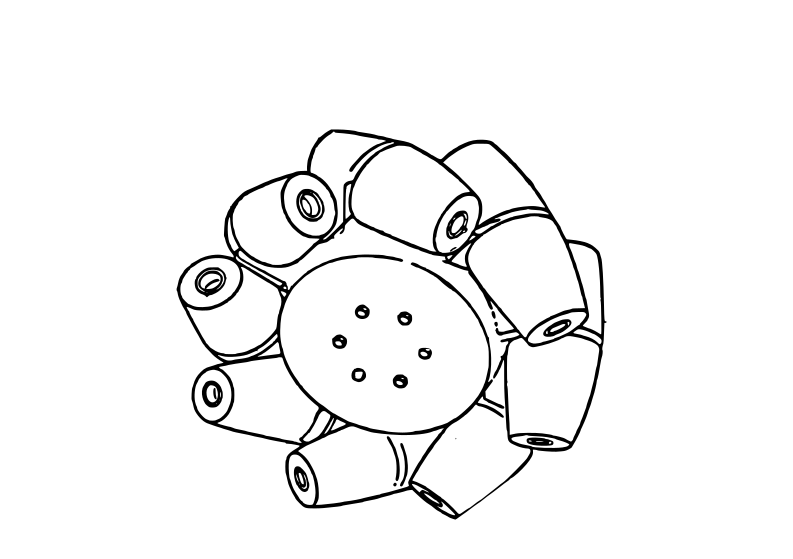
\includegraphics[width=0.4\linewidth]{mecanum_wheel.pdf}
	\caption{Side view of a Mecanum wheel~\cite{Dickerson.1991}}
	\label{fig:mecanumwheel}
\end{figure}
The rollers on a Mecanum wheel are positioned such that their axes are skewed relative to the central wheel axle. This geometry allows each wheel to produce a vector of force that, when combined with the forces generated by the other wheels, results in omnidirectional motion. This configuration avoids the singularities common in traditional wheel systems, which often require significant propulsion adjustments to perform small or intricate maneuvers. Vehicles equipped with Mecanum wheels are therefore able to perform complex maneuvers in confined spaces with greater efficiency, reducing both the time and area required for movement~\cite{Dickerson.1991}.\\
The kinematics of Mecanum wheels also play a crucial role in achieving precise control over a vehicle’s movement. As each wheel operates independently, the control system must convert the desired motion into specific commands for each wheel, accounting for the interaction between longitudinal, lateral, and rotational forces. While this may seem computationally complex, efficient algorithms have been developed to simplify the process. These algorithms, often incorporating compensation for wheel slip, ensure that the vehicle can execute smooth, omnidirectional movement without requiring significant computational overhead~\cite{Dickerson.1991}. In this case a simple control algorithm will be developed that does not use a compensation for wheel slip. As it is a fairly simple and lightweight remote controlled car for studying purposes, the required precision is not so high, that it would justify the increased development effort.\\
One notable disadvantage of the Mecanum wheel design is the inefficient transfer of kinetic energy from the motors to the ground. As the exterior rollers rotate, only a portion of the force generated by the wheels is effectively applied to the ground. This is due to the angled orientation of the rollers, which causes the total force exerted by each wheel to be split into components. Consequently, only a fraction of the force directly contributes to the vehicle’s motion, leading to reduced overall efficiency in propulsion compared to conventional wheels~\cite{F.Adascalitei.2011}.\\
Therefore, Mecanum wheels are not commonly used in applications where efficient energy use is a priority but are favored in scenarios where the efficient use of time and space is essential. Many researchers focus on utilizing these wheels in the design of autonomous vehicles~\cite{Tlale.2008} and robots, particularly for environments where maneuverability is critical. Omni-directional platforms, like those equipped with Mecanum wheels, offer the ability to move instantly in any direction from any position. This provides significant advantages in congested environments filled with static and dynamic obstacles, such as factory workshops, warehouses, hospitals, and elderly care facilities, where conventional wheeled designs would struggle to navigate narrow aisles and tight spaces efficiently~\cite{nivenb.2002}.\\

In this design, four Mecanum wheels are arranged at the four corners of a rectangular vehicle platform, with each wheel oriented to face forward along the X-axis, as can be seen in fig.~\ref{fig:mecanumwheelconfig}. 
\begin{figure}[h]
	\centering
	\captionsetup{justification=centering}
	\includegraphics[width=0.7\linewidth]{mecanum_wheel_configuration.pdf}
	\caption{Wheel configuration and coordinates of Mecanum wheel car~\cite{Dickerson.1991}}
	\label{fig:mecanumwheelconfig}
\end{figure}
The arrangement allows the vehicle to achieve omnidirectional movement, with the X-axis representing forward and backward motion, the Y-axis representing lateral (side-to-side) motion, and the $\theta$ corresponds to rotational (yaw) movement.\\ The control system uses 8-bit signed integers to define motion in each direction, with values ranging from -127 to 127 to ensure symmetry in both positive and negative directions. While 128 would be the theoretical maximum for positive values, it is capped at 127 to maintain balance with the maximum negative value of -127, thus allowing precise and symmetrical control over the vehicle’s motion in all three axes.\\
In order to achieve the desired translational movement of the vehicle along the X and Y axes (see fig.~\ref{fig:mecanumwheelconfig}), each of the four Mecanum wheels must rotate in a specific direction. The table~\ref{tab:mecanumdirection} provides a detailed breakdown of the rotational direction of each wheel corresponding to various translational movements. The wheels, designated as A, B, C, and D in the configuration, can rotate either positively, negatively, or remain idle (0) depending on the intended movement. A positive direction (+) indicates forward rotation, while a negative direction (-) refers to backward rotation. 

\begin{table}[h]
	\centering
	
	\caption{Rotation Direction for Translational Movement~\cite{Tlale.2008}}
	\begin{tabular}{c||c|c|c|c}
		\hline
		Wheel & \textbf{A} & \textbf{B} & \textbf{C} & \textbf{D} \\
		\hline
		\hline
		\textbf{Forward} & + & + & + & + \\
		\hline
		\textbf{Back} & - & - & - & - \\
		\hline
		\textbf{Left} & - & + & + & - \\
		\hline
		\textbf{Right} & + & - & - & + \\
		\hline
		\textbf{Forward-Right} & + & 0 & 0 & + \\
		\hline
		\textbf{Forward-Left} & 0 & + & + & 0 \\
		\hline
		\textbf{Back-Right} & - & 0 & 0 & - \\
		\hline
		\textbf{Back-Left} & 0 & - & - & 0 \\
		\hline
		\textbf{\acs{cw} Turn} & + & - & + & - \\
		\hline
		\textbf{\acs{ccw} Turn} & - & + & - & + \\
		\hline
	\end{tabular}
	\label{tab:mecanumdirection}
\end{table}

The precise coordination of wheel rotations enables the vehicle to move efficiently in any direction, leveraging the omni-directional capability of the Mecanum wheel design.
To translate user input into individual wheel velocities for the Mecanum wheel vehicle, a control scheme is employed that requires three signed integer values. These values correspond to the movement along the X-axis, Y-axis, and the rotational motion ($\theta$). The user provides these three inputs to control the vehicle's motion, which are represented as a 1x3 vector. This vector is then multiplied by a pre-defined translational matrix to convert the input into wheel-specific velocity values for each of the four wheels—designated A, B, C, and D. The resulting output is a 1x4 vector that determines the movement of each wheel individually. The transformation is achieved through the matrix equation~\ref{eq:mecanumtranslation}.

\begin{equation}
	\label{eq:mecanumtranslation}
	\begin{bmatrix}
		x_{val} & y_{val} & \theta_{val}
	\end{bmatrix}
	\cdot
	\begin{bmatrix}
		+1 & +1 & +1 & +1\\
		+1 & -1 & -1 & +1\\
		+1 & -1 & +1 & -1\\
	\end{bmatrix}
	=
	\begin{bmatrix}
		A & B & C & D
	\end{bmatrix}
\end{equation}
The 3x4 matrix represents the relationship between the vehicle's translational and rotational movements and the corresponding velocities of each wheel. The output vector provides the computed speed and direction for each of the four wheels.




